\documentclass[sigplan, anonymous, review]{acmart}

\usepackage{booktabs} % For formal tables


% Copyright
%\setcopyright{none}
%\setcopyright{acmcopyright}
%\setcopyright{acmlicensed}
\setcopyright{rightsretained}
%\setcopyright{usgov}
%\setcopyright{usgovmixed}
%\setcopyright{cagov}
%\setcopyright{cagovmixed}


% DOI
\acmDOI{10.475/123_4}

% ISBN
\acmISBN{123-4567-24-567/08/06}

%Conference
\acmConference[WOODSTOCK'97]{ACM Woodstock conference}{July 1997}{El
  Paso, Texas USA} 
\acmYear{1997}
\copyrightyear{2016}

\acmPrice{15.00}

%\acmBadgeL[http://ctuning.org/ae/ppopp2016.html]{ae-logo}
\acmBadgeR[http://ctuning.org/ae/ppopp2016.html]{ae-logo}


\begin{document}
\title{SIG Proceedings Paper in LaTeX Format}
\titlenote{Produces the permission block, and
  copyright information}
\subtitle{Extended Abstract}
\subtitlenote{The full version of the author's guide is available as
  \texttt{acmart.pdf} document}

\author{Ben Trovato}
\authornote{Dr.~Trovato insisted his name be first.}
\orcid{1234-5678-9012}
\affiliation{%
  \institution{Institute for Clarity in Documentation}
  \streetaddress{P.O. Box 1212}
  \city{Dublin} 
  \state{Ohio} 
  \postcode{43017-6221}
}
\email{trovato@corporation.com}

\author{G.K.M. Tobin}
\authornote{The secretary disavows any knowledge of this author's actions.}
\affiliation{%
  \institution{Institute for Clarity in Documentation}
  \streetaddress{P.O. Box 1212}
  \city{Dublin} 
  \state{Ohio} 
  \postcode{43017-6221}
}
\email{webmaster@marysville-ohio.com}

\author{Lars Th{\o}rv{\"a}ld}
\authornote{This author is the
  one who did all the really hard work.}
\affiliation{%
  \institution{The Th{\o}rv{\"a}ld Group}
  \streetaddress{1 Th{\o}rv{\"a}ld Circle}
  \city{Hekla} 
  \country{Iceland}}
\email{larst@affiliation.org}

\author{Lawrence P. Leipuner}
\affiliation{
  \institution{Brookhaven Laboratories}
  \streetaddress{P.O. Box 5000}}
\email{lleipuner@researchlabs.org}

\author{Sean Fogarty}
\affiliation{%
  \institution{NASA Ames Research Center}
  \city{Moffett Field}
  \state{California} 
  \postcode{94035}}
\email{fogartys@amesres.org}

\author{Charles Palmer}
\affiliation{%
  \institution{Palmer Research Laboratories}
  \streetaddress{8600 Datapoint Drive}
  \city{San Antonio}
  \state{Texas} 
  \postcode{78229}}
\email{cpalmer@prl.com}

\author{John Smith}
\affiliation{\institution{The Th{\o}rv{\"a}ld Group}}
\email{jsmith@affiliation.org}

\author{Julius P.~Kumquat}
\affiliation{\institution{The Kumquat Consortium}}
\email{jpkumquat@consortium.net}


% The default list of authors is too long for headers}
\renewcommand{\shortauthors}{B. Trovato et al.}


\begin{abstract}
This paper provides a sample of a \LaTeX\ document which conforms,
somewhat loosely, to the formatting guidelines for
ACM SIG Proceedings. 
\end{abstract}

%
% The code below should be generated by the tool at
% http://dl.acm.org/ccs.cfm
% Please copy and paste the code instead of the example below. 
%
\begin{CCSXML}
<ccs2012>
 <concept>
  <concept_id>10010520.10010553.10010562</concept_id>
  <concept_desc>Computer systems organization~Embedded systems</concept_desc>
  <concept_significance>500</concept_significance>
 </concept>
 <concept>
  <concept_id>10010520.10010575.10010755</concept_id>
  <concept_desc>Computer systems organization~Redundancy</concept_desc>
  <concept_significance>300</concept_significance>
 </concept>
 <concept>
  <concept_id>10010520.10010553.10010554</concept_id>
  <concept_desc>Computer systems organization~Robotics</concept_desc>
  <concept_significance>100</concept_significance>
 </concept>
 <concept>
  <concept_id>10003033.10003083.10003095</concept_id>
  <concept_desc>Networks~Network reliability</concept_desc>
  <concept_significance>100</concept_significance>
 </concept>
</ccs2012>  
\end{CCSXML}

\ccsdesc[500]{Computer systems organization~Embedded systems}
\ccsdesc[300]{Computer systems organization~Redundancy}
\ccsdesc{Computer systems organization~Robotics}
\ccsdesc[100]{Networks~Network reliability}

% We no longer use \terms command
%\terms{Theory}

\keywords{ACM proceedings, \LaTeX, text tagging}

\begin{teaserfigure}
  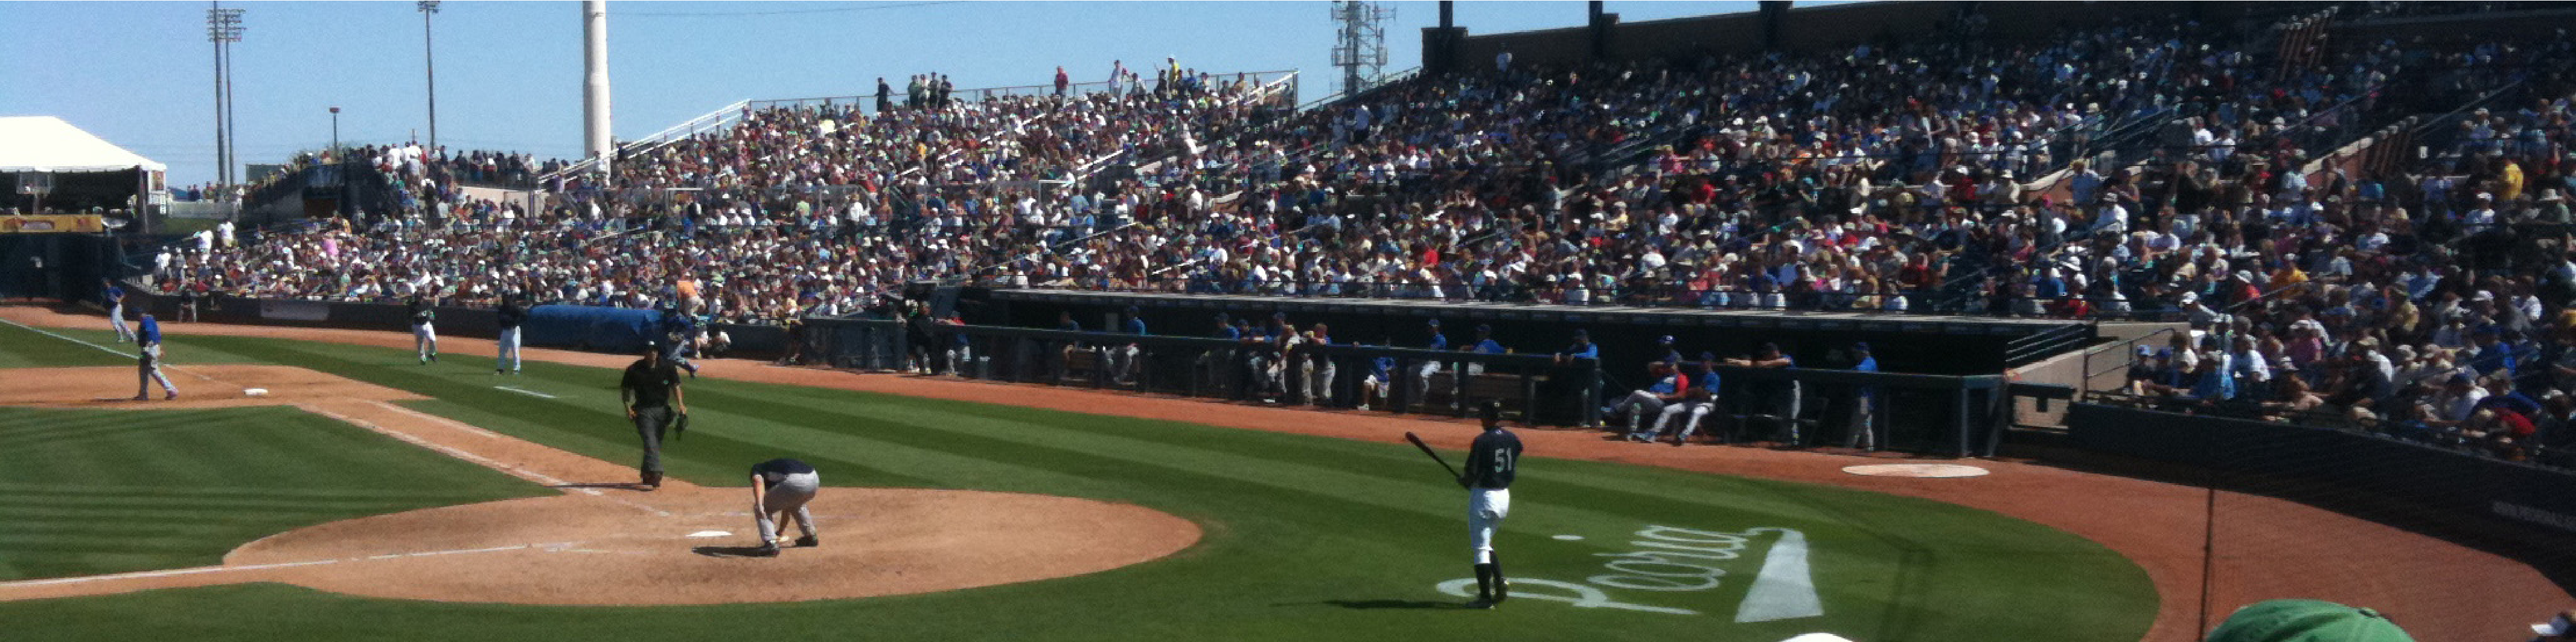
\includegraphics[width=\textwidth]{sampleteaser}
  \caption{This is a teaser}
  \label{fig:teaser}
\end{teaserfigure}


\maketitle

\section{Introduction}
There are a large number of uncertainty problems in the real world, which requires us to use prerequisite knowledge and deductive reasoning to predict the results, that is to say, to make decisions on nondeterministic problems through probability reasoning. Therefore, probabilistic programs is produced. Probabilistic programs is a kind of logic program with probabilistic facts. It makes the probabilistic reasoning model easier to build and can estimate the possibility of the expected situation.
Probabilistic programs has a wide and flexible scope of application. It is used in various fields such as business, military, scientific research and daily life. Probability is becoming more and more important in actual calculations, such as risk analysis, medical decision-making, differential privacy mechanisms~\cite{Dwork2014Differential}, etc. The analysis of programs with probability variables has also received widespread attention in academia and industry. Therefore, we need to learn the impact of probabilitisic variables on the program results, analyze and verify the properties of probabilistic grams, so as to ensure that the final results of the program have good reliability and stability.

\begin{figure}[h]
	\centering
	\begin{tabular}{ccc}
		\hline
		% after \\: \hline or \cline{col1-col2} \cline{col3-col4} ...
		program & $\rightarrow$ & typeSpecifier main\{$stmt^*$\} \\
		stmt & $\rightarrow$ & assign | condStmt | while \\
		assign & $\rightarrow$ & intAssign | realAssign \\
		condStmt & $\rightarrow$ & ifStmt | ifElseStmt\\
		while & $\rightarrow$ & while (test) $stmt^*$\\
		intAssign & $\rightarrow$ &  intVar=intConst | intVar $\sim$ intRandom\\
		realAssign & $\rightarrow$ & realVar=realConst | realVar $\sim$ realRandom\\
		intRandom & $\rightarrow$ & uniformInt(intConst,intConst)\\
		&  & | Bernoulli(intConst,intConst)\\
		&  & $\cdots$ \\
		realRandom & $\rightarrow$ & uniformReal(realConst,realConst)\\
		&  & | Gaussian(realConst,realConst)\\
		&  & $\cdots$ \\
		intExpr & $\rightarrow$ & intConst | intRandom | intExpr$\pm$intExpr\\
		& & intConst * intExpr| intExpr/intConst\\
		realExpr & $\rightarrow$ & realConst | realRandom | realExpr$\pm$realExpr\\
		& & realConst * realExpr| realExpr/realConst\\
		boolExpr& $\rightarrow$ & true | false | boolExpr $\wedge$ boolExpr \\
		& & intExpr relop intExpr | realExpr relop realExpr\\
		relop & $\rightarrow$ & <  |> | $\geq$ | $\leq$ | ==\\
		\hline
	\end{tabular}
	\label{syntax}
	\caption{Partial syntax specification of probabilistic programs language}
\end{figure}

This paper presents a verification tool PMars based on probabilistic programs, which can automatically analyze probabilistic language conforming to the specification (As shown in Figure \ref{syntaxy}). It mainly includes two parts: one is to estimate the correct probability interval of given assertion when the program terminates; the other is to analyze the termination qualitatively and quantitatively.


More specifically, probabilistic programs validates tool PMars provides:
\begin{enumerate}
	\item Define and parse probabilistic programs language. More than ten kinds of probability distributions are built in, which is convenient to call for building probabilistic model.
	\item Reduce the estimation of given assertions to polyhedron solving problem. In addition, we support the probabilistic programs of infinite state.
	\item Reduce the termination analysis to linear programming problem. We also consider the concentration results under the premise that the program can be terminated.
\end{enumerate}

\section{Probabilistic Programs}

In order to analyze and verify probabilistic programs, we first need a probabilistic language with sufficient expressivity and easy to understand. We now consider the syntax~\cite{Minka2012Compiler} of probabilistic programs, whose syntax specifications are shown in Figure \ref{syntax}. The expressions in the probabilistic language is similar to the classic imperative programs, mainly composed of three statements: assignment statement, condition-branch statement (if-else) and loop statement (while). In addition, a variety of random value generators are built-in, as shown in Figure \ref{distribution}, which can be used to simulate different distribution situations. Variables are classified into two types: program variables and sampling variables. Program variables include integer variables, real variables and boolean variables. Boolean variables are mainly used for condition statement and loop statement. Sampling variables is assigned to when the program is running, which is subject to a continuous probability distribution or discrete probability distribution.

\newcommand{\tabincell}[2]{\begin{tabular}{@{}#1@{}}#2\end{tabular}}
\begin{table}[htb]
	\caption{Specification of the inbuilt random value generators}
	\label{distribution}
	\begin{tabular}{lll}  
		\toprule   
		Name & Parameter & \makebox[4cm][c]{Density Function} \\  
		\midrule   
		R($\mathbb{X},\mathbb{P}$) & $\sum\limits_{n=1}^N p_n$=1 & $P(X=x_k)=p_k$\\  
		Binomial(n,p) & \tabincell{c}{0<p<1\\n$\geq$1} &$\tbinom{k}{n}p^k(1-p)^{n-k}, k=1,2,\dots$ \\  
		Poisson($\lambda$) & $\lambda$>0 &$\frac{\lambda^ke^{-\lambda}}{k!}$ \\   
		UnifInt(a,b) & a$\leq$b & 
		$\left\{
		\begin{array}{lr}
			\frac{1}{b-a} &, b>a \\
			1 & ,a=b\\
		\end{array}
		\right.$ \\
		UnifReal(a,b) & a<b & $\frac{1}{b-a}$ \\  
		Exponential($\theta$) & $\theta$>0 & $\frac{1}{\theta}e^{\frac{x}{\theta}}$ \\    
		Normal($\mu$,$\sigma^2$) &$\sigma$>0 &$\frac{1}{\sqrt{2\pi}\sigma}e^{-(x-\mu)^2/(2\sigma^2)}$ \\
		Gamma($\alpha$,$\beta$) & $\alpha, \beta$>0 & 
		$\frac{1}{\beta^\alpha\Gamma(\alpha)}x^{\alpha-1}e^{\frac{-x}{\beta}} , x>0 $  \\  
		Beta($\alpha$,$\beta$) & $\alpha, \beta$>0 & $\frac{\Gamma(\alpha+\beta)}{\Gamma(\alpha)\Gamma(\beta)}x^{\alpha-1}(1-x)^{\beta-1}$,0<x<1\\    
		Laplace(x|$\mu,\lambda$) & $\lambda>0$ &$\frac{1}{2\lambda}e^{\frac{|x-\mu|}{\lambda}}$ \\
		Geometric(p) & 0<p<1 & $(1-p)^{k-1}p, k=1,2,\dots$ \\     
		T(n) &n$\geq$1 &$\frac{\Gamma(\frac{n+1}{2})}{\sqrt{n\pi}\Gamma(\frac{n}{2})}(1+\frac{x^2}{n})^{-(n+1)/2}$ \\
		\bottomrule  
	\end{tabular}
\end{table}

We use control flow graphs (CFGs) to express the semantics of probabilistic programs~\cite{Kozen1981Semantics}. It is a tuple which takes the form (L,(X,R),$\mapsto$,$\bot$), where:

\begin{itemize}
\item L is a finite set of labels L=\{$\ell$$_0$,$\ell$$_1$,\dots,$\ell$$_n$\} that represent the control locations. Each statement in a program has a unique label. Such as $\ell$$_0$ indicates the starting location, $\ell$$_n$ indicates the last location.

\item (X,R) is a set of variables, where X=\{x$_0$,\dots,x$_n$\} is the set of program variables and R=\{r$_1$,\dots,r$_m$\} is the set of sampling variables.

\item $\mapsto$ is a transition relationship. $\ell$$_i$ is equivalent to a node in the control flow graph and $\mapsto$ is equivalent to transition from one node to another node. It can be expressed in the form of ($\ell$,$\alpha$,$\ell$').

\item $\bot$ is a sign of the exit of the program.
\end{itemize}

\section{Estimating the probabilities of assertions}
The goal of this section is to estimate the probability that a given assertion is correct at the exit of the program. There are two main steps.


The First step is to generate sufficient and appropriate path set S with high confidence coverage. The finite set $S=\{s_1,\dots,s_i,\dots,s_n\}$ contains distinct paths that can be terminated, where $s_i: \ell_0 \to \dots \to \ell_k \to \dots \to \ell_{\bot}$. The control flow of loop statements on program variables and sampling variables may put the program in infinite state. Therefore, we adopt the method of simulating symbol execution. Execution paths can be represented as a tree. Through symbol execution~\cite{Geldenhuys2012symbolic}, we traverse the program execution tree and collect the semantic state. So that each path of the program execution is based on the original probability distribution. In this way, our method is able to solve the problem even if program P contains program variables and sampling variables with a wide rang of distribution or even infinite state. We need to improve the coverage c of path set S to all paths in a finite time. Estimating the probability of a given assertion $\varphi$ on path set S can be considered approximately as a whole program. We refer to some papers~\cite{Sankaranarayanan2013Static} that show the coverage c can be considered to be at least $95\%$ with 99\% confidence, when no new path is generated in 90 consecutive iterations.


The second step is to estimate the probability of a given assertion $\varphi$. For the path set S collected above, we can analyze each path in turn, then estimate the path probability and the assertion probability. Due to the calculation of accurate probability is closely related to volume of n-dimensional convex polyhedron. When the dimension increases, the calculation becomes more difficult and the time complexity is high~\cite{Arora1998Proof}. Usually, it will fail due to the calculation or insufficient memory. On the premise of weighing the efficiency and accuracy of calculation, we focus on calculating the probability interval of given assertion rather than estimated value.

\begin{algorithm}
	\caption{mcBoundProbability}
	\label{mcBoundProbability}
	\begin{algorithmic}[1]
		\REQUIRE Polytop p=(vars,constraints), maxDepth
		\ENSURE Probability interval[p1,p2]
		\IF{isABox() || maxDepth<=0}
			\STATE [p1,p2]+=computeBoundingProbability();
		\ENDIF  \\
		$//$ If at least two (or more) non trivial clusters remain, then perform the
		decomposition.  
		\IF{isDecomposable(p)}
			\STATE dim=selectBranchDimension();
			\STATE branches=branchAndBound(dim,nBranch);
			\FOR{b in branches}
			\STATE mcBoundProbability(b,maxDepth-1);
			\ENDFOR
		\ENDIF
	\end{algorithmic}
\end{algorithm}

Path probability. Each path has a series of variables and constraints. We need to estimate the probability of satisfying all constraints given the probability distributions on variables. Each variable can be regarded as a dimension of convex polyhedron. The probability problem can be reduced to polyhedron solving problem~\cite{Visser2012Green}. However, the solution of convex polyhedron by linear programming is too rough. Let us first decompose convex polyhedron into several non-intersecting convex bodies~\cite{Bingsheng2020} and then add up the calculation results. As described in Algorithm \ref{mcBoundProbability}, the isDecomposable() function is used to determine whether it can be decomposed. If true, it will be decomposed along the selected dimension. When the boundary box is found, the upper and lower bounds will be calculated by computeBoundingProbability() function. Based on the idea of importance sampling, selectBranchDimension() function selects a dimension which is unbounded or half bound or else select max width dimension. The branchAndBound() function decomposes according to the selected dimension, nBranch is the number of segmentation, the default is 2. In addition, to avoid infinite decomposition, we set maxDepth as the maximum recurrence depth, and our project is set as 12. Each path is calculated by the Algorithm \ref{mcBoundProbability}. Because there is no intersection of each path, the path probability is equal to the sum of the each paths' probability. Let's assume the assertion probability is $[p_1,p_2]$. It indicates that the maximum 1-$p_1$ path has not been explored. This will be used to calculate the upper of assertion probability.


Assertion probability. The method of assertion probability is the same as path probability, also refer to Algorithm \ref{mcBoundProbability}. The only difference is need to add assertion $\varphi$ to conditional constraints. Let's assume the assertion probability is $[q_1,q_2]$. However, the path set S can't cover all paths in the program. We need to consider the probability of unexplored paths and add the probability beyond the path set S to the upper bound of assertion probability. Then the probability interval of given assertion is $[q_1,q_2+(1-p_1)]$.

\section{Termination Analysis}
Termination analysis~\cite{Codish1999Semantic} is an important part of program verification. Ensuring that the termination is a necessary condition for the correct verification of probabilistic program. In order to solve this problem, We have referred to some papers~\cite{kris2016termination,
	cha2015algorithmic, Hermanns2013Probabilistic}. Decided to choose a powerful method to prove the termination of the probabilistic programs. That is, based on the concept of ranking supermartingale~\cite{Chakarov2013Martingales} analyze the probabilistic program qualitatively and quantitatively. Detailed as Algorithm \ref{TA}

\begin{algorithm}[htb]  
	\caption{Termination Analysis.}  
	\label{TA}  
	\begin{algorithmic}[1]  
		\REQUIRE 
		Program P; 
		\ENSURE  
		Judge whether the program is terminated, isT;\\
		The probability to terminate afer N steps decreases exponentially, N;
		\STATE Set quadratic template $g(\ell,\boldsymbol{x})$. Each location has the common template with unique coefficient. If $\ell_{\bot}$, the template g=K.
		\STATE Traverse the programs parse tree and collect the invariant I[] for each location.
		\STATE Calculate the Pre-Expectation for each location.\\
		\quad \quad case "assignment statement" :\\
		\quad \quad \quad \quad $pre(\ell,\boldsymbol{x})= \mathbb{E}(g(\ell',f(\boldsymbol{x},\boldsymbol{r})),\boldsymbol{x})$.\\
		\quad \quad case "condition(if-else) or loop(while) statement" :\\
		\quad \quad \quad \quad $pre(\ell,\boldsymbol{x})=g(\ell',\boldsymbol{x})$.\\
		\quad \quad case "terminal statement" :\\
		\quad \quad \quad \quad $pre(\ell,\boldsymbol{x})=g(\ell,\boldsymbol{x}).$
		\STATE According to the concept of half-space, $H=g(\ell,\boldsymbol{x})-pre(\ell,\boldsymbol{x})-\epsilon$
		\STATE According to the concept of Handelman's Theorem, $H'=\sum\limits_{i=1}^{d} a_i\cdot I_i$, where $\mu=\{\prod\limits_{i=1}^{2}\nu\}$ $a_i$ is a non-negative real number.
		\STATE Pattern extraction. The coefficient of H corresponds to that of H', which is converted into linear programming. If solvable, the program P can be terminated, otherwise return.
		\STATE Calculate the difference-bounded [a,b] $(a\leq g(\ell',\boldsymbol{x})-g(\ell,f(\boldsymbol{x},\boldsymbol{r}))\geq b)$
		\STATE Obtain N, according to $\mathbb{P}(\bm{T_p} > N) \leq e^{-\frac{2(\epsilon(N-1)-g(\ell_0,x_0))^2}{(N-1)(b-a)^2}}$
	\end{algorithmic}  
\end{algorithm}  


Qualitative analysis. It mainly analyzes whether the probabilistic programs will be terminated with probability 1 (almost sure termination)~\cite{Hurd2002A}. The specific idea is to calculate the supermartingale of each location and the value of location $\ell$' does not exceed the location $\ell$. Refer to Algorithm \ref{TA} step 1 to 6. Supermartingales are represented by template g with a natural number as the maximal degree. For the sake of simplicity, our tool takes 2, that is, the template g is a quadratic equation. Then calculate Pre-Expectation according to the formulas of step 3, where $\ell$' is the next location of $\ell$ and $f$ is the transition relation from location $\ell$ to $\ell$'. We know that Pre-Expectation belong to convex set. The definition of half-space $\{x|\textbf{a}^T\textbf{x}\leq b\}$ can be transformed into $\{x|(\textbf{c}^\ell)^T\textbf{x} \leq d^\ell-\epsilon\}$ and $c^\ell,d^\ell$ is a vector / scalar linear expression related to pre($\ell,\boldsymbol{x}$). we will apply it to Pre-Expectation, it is equivalent to $pre(\ell,\boldsymbol{x}) \leq g(\ell,\boldsymbol{x})-\epsilon$, and $\epsilon$ takes 1. Finally, according to Handelman's theorem, we can transform this problem into linear programming.

\begin{table*}[pt] 
	\caption{Experimental results:Termination Analysis}  
	\label{TerminationResult} 
	\begin{center}  
		\begin{tabular}{|l|l|l|l|l|}  
			\hline  	
			Example & $x_0$ & g($\ell_0,x_0$) & UB(P) & N\\ \hline  	
			Simple & $x=100$  & 6x+2 & 603 & 2670 \\ \hline  		
			NestedLoop & $x=1$ & 1040x+2290 & 1251 & 382807 \\  \hline  
			Award & bonus=0 & -4.0$\cdot$bonus+442& 443 &10658 \\  \hline  
			RandomWalk & $position=0$ & -20$\cdot$position+122 & 123 & 11937 \\  \hline  
			Gambler& $money=3$ & 400$\cdot$money+402& 1603 & 3641131 \\ \hline  		 
			Gambler2 & $money=10$ & 45.454545$\cdot$money+456.545455 & 913 & 3134301 \\  \hline  
			Bitcoin mining & $coin=10$ & 5.317601$\cdot$coin+2 & 57 & 1.532647E8 \\  \hline 
			Infection & x=1000, $p_1$=0.25, $p_2$=0.1, q=0.3 & 21.107713+0.038215x+$6.6E-5x^2$& 59 & 215 \\  \hline  
		\end{tabular}  
	\end{center}  
\end{table*}

Quantitative analysis. Calculate the boundary N, so that the probability program concentrates on terminating before N steps. That is, the probability of termination after N steps shows an exponential decreases. We focus on the approximating of the expected termination time, refer to Algorithm \ref{TA} step 7 to 8. According to the previous steps, we can find the coefficients of polynomial template. If we know the initial value of variables, we can know that the first location is g($\ell, x_0$), the terminated location $\ell_\bot$ is K and the difference between each location is $\epsilon$. For verification tool for probabilistic programs PMars, the value of K is -1 and the value of $\epsilon$ is 1. Therefore, when program P can be almost sure terminated, we can get the upper bound on termination time for the given initial condition is ET(P) $\leq$ UB(P) = $\frac{g(\ell, x_0)-K}{\epsilon}$.  Exponential sum is one of the most commonly used specific function families in nonlinear approximation theory. Our main idea is based on martingale inequality of Azuma's Inequality, Hoeffding's Inequality and Bernstein's Inequality. In probability theory, the Azuma's inequality gives a concentration result for the values of martingales that have bounded differences. Hoeffding's Inequality~\cite{Hoeffding1963} is a special case of Azuma's Inequality. It proposes an upper bound on the probability that the sum of random variables deviates from its expected value. Bernstein's Inequality is a generalization of Hoeffding. It can handle not only independent variables but also weak independent variables. Derivation from the paper~\cite{cha2015algorithmic}, We know when $\epsilon(N-1) > g(\ell_0,\boldsymbol{x_0})$, then $\mathbb{P}(\bm{T_p} > N)\leq e^{-\frac{2((N-1)-g(\ell_0,x_0))^2}{(N-1)(b-a)^2}}$. Given the exponent, we can get the result of N.


\section{Experimental Results}
In this section, we present our experimental results. For all the examples, you can view it on GitHub.


Table \ref{AssertionsResults} presents the experimental results about estimating the probabilities bounds of assertions, where 'Assertion' is a Boolean expression, it can contain addition and subtraction operations and it also support the use of logical operator \&\&, 'c' is the lower bound of path coverage, 'Bounds' is the upper and lower bounds of the given assertion. Due to layout restrictions, some values are not presented in the table, such as the total number of execution paths and unique paths.

\begin{table}[htb]   
	\caption{Experimental results: Estimating the probabilities bounds of assertions}
	\label{AssertionsResults} 
	\begin{tabular}{c |c |c |c }
		\hline  
		Ex. & Assertion &  c & Bounds \\ \hline
		\multirow{2}{*}{carton}
		& count$\geq$5 & 0.9485 & [0.948540,1] \\ \cline{2-4}
		& count$\geq$10 & 0.9539, & [0.000639,0.046711] \\ \cline{2-4}
		& count$\leq$7 & 0.9549 & [0.918762,0.963832] \\ \cline{2-4}
		& totalWeight$\geq$5.5 & 0.9386 & [0.382145,0.453010] \\ \cline{2-4}
		& totalWeight$\geq$6 & 0.9428 & [0.246186,0.342997]  \\ \hline
		\multirow{2}{*}{herman}
		& count$\geq$1 & 0.9561 & [0.581128,0.625000] \\ \cline{2-4}
		& count$\geq$20 & 0.9701 & [0.000000,0.029876]  \\ \hline
		\multirow{3}{*}{\makecell[c]{framin\\gham}}
		& points$\geq$10 & 0.9636 & [0.137343,0.173695] \\ \cline{2-4}
		& pointsErr-points$\geq$5 & 0.9365 & [0.778149,0.849318]  \\ \cline{2-4}
		& points-pointsErr$\geq$5 & 0.9326 & [0.177619,0.246763]  \\ \hline
		\multirow{5}{*}{\makecell[c]{sum-\\three}}
		& x+y>z+10& 0.9886 & [0.447672,0.470723] \\ \cline{2-4}
		& x+y+z>8 & 0.9886 & [0.454482,0.475890] \\ \cline{2-4}
		& x+y+z>100 & 0.9886 & [0.012422,0.025870]  \\ \cline{2-4}
		& x>5 \&\& y>0& 0.9886 & [0.150535,0.163590]  \\ \cline{2-4}
		&  \makecell[c]{x>0 \&\& y>0 \\ \&\& z>0} & 0.9886 & [0.125582,0.137293] \\ \hline
		\multirow{1}{*}{ckd-epi}
		& f -f1$\geq$0.1 & 0.9252 & [0.351632,0.426397] \\ \cline{2-4}
		& f1 -f$\geq$0.1 & 0.9261 & [0.387275,0.461157]  \\ \hline
	\end{tabular}  
\end{table}

We have written some simple but classical probabilistic programs with 'while' loop-statements. In Table \ref{TerminationResult}, we present the experimental results about termination analysis, where '$x_0$' means the initial value of variable, 'g($\ell_0,x_0$)' is the polynomial ranking supermartingale about the starting location, 'ET(P)' is the upper bound of expected termination time and 'N' is the bound that the probability of termination after N steps shows an exponential decreases (we set the exponent to 1.5 $\cdot 10^{-5}$).

\section{Conclusions and Future Work}
At present, uncertainty exists in many software systems, including data analysis, stochastic algorithm and Monte Carlo simulation. The design of PMars tool is to provide convenience and method for inference problem of probabilistic program system. PMars defines the basic syntax with probability distribution, which is used to model of probabilistic programs. PMars can collect path set S with high confidence coverage and calculate probability interval and assertion probability interval of each path. In addition, based on the idea of ranking-supermartingales, PMars can also perform qualitative and quantitative analysis on the termination of probabilistic programs.


However, we have only solved some aspects of the complex problem of probabilistic programs analysis and verification. We still have some areas for improvement:
\begin{enumerate}
	\item Limited to linear program. PMar can't deal with the cases of variable multiplication, division and exponents, etc., regardless of the estimation of the assertion probability interval or the termination analysis,
	\item Non-deterministic probabilistic programs is not supported. PMars can handle random variables with know probability distribution and probabilistic transitions. But for programs with uncertain variables and non-deterministic transitions, it can't handle them.
	\item We hope to find a better way to get more accurate probability interval under the premise of ensuring efficiency. 
\end{enumerate}

%\end{document}  % This is where a 'short' article might terminate



\appendix
%Appendix A
% \section{Headings in Appendices}

% \subsection{Introduction}
% \subsection{The Body of the Paper}
% \subsubsection{Type Changes and  Special Characters}
% \subsubsection{Math Equations}
% \paragraph{Inline (In-text) Equations}
% \paragraph{Display Equations}
% \subsubsection{Citations}
% \subsubsection{Tables}
% \subsubsection{Figures}
% \subsubsection{Theorem-like Constructs}
% \subsubsection*{A Caveat for the \TeX\ Expert}
% \subsection{Conclusions}%

% This next section command marks the start of
% Appendix B, and does not continue the present hierarchy

\begin{acks}


\end{acks}


\bibliographystyle{ACM-Reference-Format}
\bibliography{sigproc} 

\end{document}
